%
% chapter.tex -- Kapitel über Eigenwerte
%
% (c) 2018 Prof Dr Andreas Müller, Hochschule Rapeprswil
%
\chapter{Eigenwerte und Eigenvektoren\label{chapter-eigen}}
\lhead{Eigenwerte und Eigenvektoren}
\rhead{}
\index{Eigenwert}
\index{Eigenvektor}
\rhead{Eigenwerte und Eigenvektoren}
In vielen Anwendungen hat man ein Gleichungssystem der Form
\[
Ax=\lambda x
\]
zu lösen, wobei nicht nur der Spaltenvektor $x$, sondern auch der
Parameter $\lambda$ unbekannt sind.
Natürlich kann man ein solches Problem immer umschreiben in die Form
\[
(A-\lambda E) x=0,
\]
also ein Gleichungssystem, welches entweder gar keine, oder dann
unendlich viele Lösungen hat.
Daher interessiert die Frage 
ganz besonders, für welche $\lambda$ eine nicht triviale Lösung möglich ist.

In diesem Kapitel geht es darum, diese sogenannten Eigenwerte $\lambda$
und die zugehörigen Lösungsvektoren, die Eigenvektoren, zu finden.
Dieses
Problem ist von grosser praktischer Bedeutung, sehr viele Anwendungsproblem
lassen sich darauf zurückführen.
Es lohnt sich also, dieses Problem
effizient lösen zu können.
Beispiele:
\begin{compactitem}
\item Lösung von linearen Differenzengleichungen
\index{lineare Differenzengleichung}
\item Lösung von linearen Differentialgleichungen beliebiger Ordnung
\index{lineare Differentialgleichung}
\item Schwingungen eines Bauwerks oder einer Maschine: die Bewegung wird durch
eine partielle Differentialgleichung beschrieben, die Schwingungsfrequenzen
werden durch die Eigenwerte gegeben.
Um Resonanzen und damit die Zerstörung
zu verhindern, muss der Ingenieur die Eigenfrequenzen
berechnen können.
\index{Schwingung}
\index{Eigenfrequenz}
\item Resonanzen eines Hohlraumresonators: die Felder im Hohlraumresonator
werden durch eine partielle Differentialgleichung beschrieben.
Die Eigenfrequenzen sind Eigenwerte, der Ingenieur kann durch Veränderung
der Geometrie des Hohlraumes das Frequenzspektrum anpassen.
\index{Resonanz}
\index{Hohlraumresonator}
\index{partielle Differentialgleichung}
\index{Frequenzspektrum}
\item
\index{Akustik}
In der
Akustik strebt man eine möglichst gleichmässige Verteilung der Eigenfrequenzen
eines Konzertsaals an, um dem Zuhörer ein möglichst ausgewogenes Klangbild
zu bieten.
\item Klangspektrum eines Musikinstruments: Die Schwingungen eines Musikinstruments
werden durch eine partielle Differentialgleichung beschrieben, die
Eigenwerte beschreiben die Oberton-Frequenzen, die im Klangspektrum des
Instruments vertreten sind.
\index{Klangspektrum}
\end{compactitem}
Bis auf das erste Beispiel stehen Ihnen die mathematischen Mittel noch nicht
zur Verfügung, auch nur die Problemstellung zu formulieren, daher beginnen
wir mit einer Differenzengleichung als einführendes Beispiel.

%
% problem.tex
%
% (c) 2018 Prof Dr Andreas Müller, Hochschule Rapperswil
%
\section{Problemstellung}
In diesem Kapitel gehen wir immer von einer $n\times n$-Matrix $A$ aus.

\medskip
{\parindent0pt \bf Problem:} Finde Vektoren $x\in\mathbb R^n$ und
Zahlen $\lambda\in\mathbb R$ so, dass $Ax=\lambda x$.
\medskip

{\parindent0pt Diese Problemstellung ist nicht ganz klar:}
\begin{compactitem}
\item Der Vektor $x=0$ ist immer eine Lösung, das Problem ist also
nur dann interessant, wenn Vektoren $x\ne 0$ verlangt werden.
\item Der Vektor $x$ ist nicht eindeutig bestimmt.
Gilt $Ax=\lambda x$, dann gilt dasselbe auch für $y=\mu x$:
\[
Ay= A(\mu x)=\mu Ax=\mu\lambda x = \lambda (\mu x)=\lambda y.
\]
Der Vektor $x$ kann also bestenfalls bis auf ein Vielfaches bestimmt werden.
\end{compactitem}

\index{Eigenwert}
\index{Eigenvektor}
\begin{definition}
Ein Vektor $v \in \mathbb R^n$ heisst Eigenvektor der $n\times n$-Matrix $A$
zum Eigenwert $\lambda$, wenn $v\ne 0$ und $Av=\lambda v$ gilt.
\end{definition}

\begin{beispiel}
Die Matrix
\[
\begin{pmatrix}
3&0&0\\
0&5&0\\
0&0&7
\end{pmatrix}
\]
hat die Eigenwerte $3$, $5$ und $7$, mit den Eigenvektoren
\[
\begin{pmatrix}
1\\0\\0
\end{pmatrix}
,
\begin{pmatrix}
0\\1\\0
\end{pmatrix}
,
\begin{pmatrix}
0\\0\\1
\end{pmatrix}
\]
\end{beispiel}

\begin{hilfssatz}
\index{Diagonalmatrix}
Die Diagonalmatrix
\[
\operatorname{diag}(\lambda_1,\dots,\lambda_n)
=\begin{pmatrix}
\lambda_1&\dots&0\\
\vdots&\ddots&\vdots\\
0&\dots&\lambda_n
\end{pmatrix}
\]
hat die Eigenwerte $\lambda_1,\dots,\lambda_n$, die Standardbasisvektoren
$e_i$ sind Eigenvektoren zum Eigenwert $\lambda_i$.
\end{hilfssatz}
Offenbar ist dies ein besonders einfacher Fall, die Basisvektoren sind
alle Eigenvektoren.
Es gibt einige Klassen von Matrizen, bei denen es
immer möglich ist, eine Basis aus Eigenvektoren zu wählen.
Hat die
$n\times n$-Matrix $A$ $n$ linear unabhängig Eigenvektoren $v_1,\dots,v_n$
mit Eigenwerten $\lambda_1,\dots,\lambda_n$, dann kann man die Wirkung
der Matrix $A$ auf einen beliebigen Vektor $x=\alpha_1v_1+\dots+\alpha_nv_n$
sofort berechnen:
\[
Ax=\alpha_1Av_1+\dots+\alpha_nAv_n=\alpha_1\lambda_1v_1+\dots+\alpha_n\lambda_nv_n.
\]
In der Basis $\{v_1,\dots,v_n\}$ hat $A$ also die Matrix
\[
A=\operatorname{diag}(\lambda_1,\dots,\lambda_n)
=
\begin{pmatrix}
\lambda_1&\dots&0\\
\vdots&\ddots&\vdots\\
0&\dots&\lambda_n
\end{pmatrix}.
\]
\begin{definition}
\index{diagonalisierbar}
\index{diagonalisieren}
Eine Matrix $A$ heisst diagonalisierbar, wenn es eine Basis aus
Eigenvektoren gibt.
\end{definition}

Wir haben also die Gleichung $Ax=\lambda x$ zu lösen.
Wäre $\lambda$ bekannt, könnten wir das Problem in ein Standardproblem
umwandeln:
\[
Ax=\lambda x\qquad\Rightarrow\qquad Ax-\lambda Ex=(A-\lambda E)x=0
\]
gesucht ist also ein nicht verschwindende Lösung des homogenen
Gleichungssystems mit
Matrix $A-\lambda E$.
Nur kennen wir $\lambda$ nicht.
Allerdings
liefert gerade die Bedingung, dass wir ein nicht verschwindende
Lösung des homogenen Systems finden wollen, ein Kriterium zur
Bestimmung von $\lambda$: $A-\lambda E$ muss singulär sein.
Das Eigenwertproblem wird also in zwei Schritten gelöst:
\begin{compactenum}
\item Bestimmung der möglichen Eigenwerte: für welche Werte von $\lambda$
ist $A-\lambda E$ singulär?
\item Bestimmung der Eigenvektoren zu gegebenem Eigenwert: Finde die
Lösungen von $(A-\lambda E)x=0$.
Hierzu kann der Gauss-Algorithmus
verwendet werden, oder in einfachen Fällen auch die Cramersche Regel.
\end{compactenum}
Die folgenden Einführungsbeispiele sollen zeigen, wie das Eigenwertproblem
in der Praxis auftaucht und gelöst werden kann.


%
% beispiele.tex
%
% (c) 2020 Prof Dr Andreas Müller, Hochschule Rapperswil
%
\subsection{Beispiele
\label{subsection:qam:beispiele}}
Die Quadratur-Amplituden-Modulation ermöglicht, im Vergleich zur
Trägerfrequenz langsam veränderliche zweidimensionale Signale zu
übertragen und wieder zu rekonstruieren.
Der besondere Nutzen dieser Technik ist jedoch, dass sie viele
ältere Modulationsverfahren als Spezialfälle enthält, wie in
diesem Abschnitt gezeigt werden soll.

\subsubsection{Amplitudenmodulation}
{\em Amplitudenmodulation} konnten wir verstehen, bevor wir $Q(t)$ kannten,
sie ist der Spezialfall $Q(t)=0$.
Für ein Audiosignal $A(t)$ mit $A(t)<1$ wird $I(t)=1+A(t)$ verwendet.
Das in Europa weitgehend bereits durch Digitalradio ersetzte 
Mittelwellenradio (AM) verwendet Amplitudenmodulation.
Bis 2025 werden in Europa alle Radiostationen digitalisiert, damit
wird AM für den Rundfunk aussterben.

\subsubsection{Phasenmodulation}
\begin{figure}
\centering
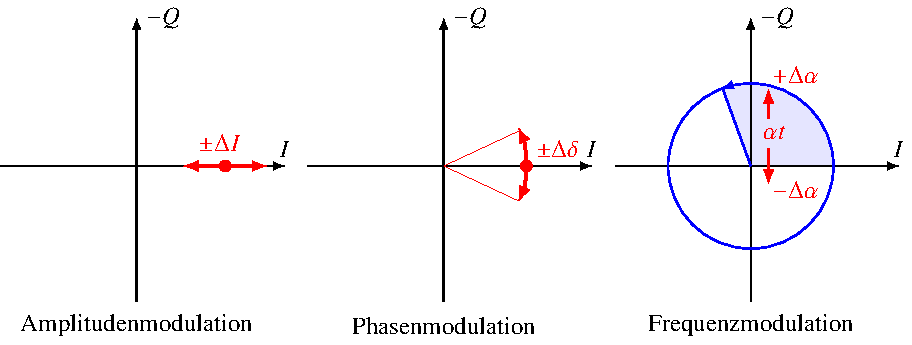
\includegraphics{applications/qam/images/amfmpm.pdf}
\caption{Amplitudenmodulation (links), Phasenmodulation (mitte) und
Frequenzmodulation in der $I$-$Q$-Ebene.
Frequenzmodulation ensteht durch eine Drehung in der $I$-$Q$-Ebene
mit der Kreisfrequenz der gewünschten Frequenzänderung.
\label{qam:figure:amfmpm}}
\end{figure}
Statt der Amplitude kann auch die Phase des Trägersignals moduliert werden.
Dazu muss $\omega t$ ersetzt werden durch $\omega t + \delta$.
Der konstante unmodulierte Vektor $\vec{v}_0$ in der $I$-$Q$-Ebene erzeugt
das modulierte Signal
\begin{align*}
D_{\omega t + \delta}
\vec{v}_0
&=
D_{\omega t}\underbrace{D_{\delta} \vec{v}_0}_{\displaystyle=\vec{v}(t)}.
\end{align*}
Eine Phasenänderung um den Winkel $\delta$ entsteht also dadurch, dass
man den Vektor $\vec{v}_0$ in der $I$-$Q$-Eben um $\delta$ dreht.
Dieses Modulationsverfahren heisst {\em Phasenmodulation}.
Abbildung~\ref{qam:figure:amfmpm} zeigt in der Mitte die Transformation
in der $I$-$Q$-Ebene, die Phasenmodulation bewirkt.

Mit reiner Amplitudenmodulation lässt sich kein Stereosignal übertragen.
Sind $L(t)$ und $R(t)$ die beiden Stereokanäle, dann erfolgt die
Amplitudenmodulation typischerweise mit $I(t)=1+L(t)+R(t)$,
wobei man wieder $L(t)+R(t)<1$ voraussetzen muss.
Ein reiner AM-Empfänger wird also nur das Audio-Signal $A(t)=L(t) + R(t)$
empfangen.

Um die Stereoinformation zu übermitteln, muss zusätzlich die Differenz
$L(t)-R(t)$ übermittelt werden.
Das C-QUAM Verfahren ({\bf C}ompatible {\bf Qu}adrature {\bf A}mplitude
{\bf M}odulation) verwendet dafür $Q(t)=L(t)-R(t)$.
Man darf annehmen, dass $L(t)-R(t)$ klein ist.
Dann befinden sich die Punkte $(I(t),Q(t))$ immer in der
Nähe der $I$-Achse, was sich in einer kleinen Verschiebung
\[
\delta = \arctan\frac{Q(t)}{I(t)} = \arctan\frac{L(t)-R(t)}{1+L(t)+R(t)}
\]
der Phase des übermittelten Signals äussert.
Der Betrag des Vektors $\vec{v}(t)$ ist dagegen
\begin{align*}
|\vec{v}(t)|
&=
\sqrt{
(1+L(t)+R(t))^2
+
(L(t)-R(t))^2
}
=
(1+L(t)+R(t))
\sqrt{
1+
\biggl(
\frac{L(t)-R(t)}{1+L(t)+R(t)}\biggr)^2
}
\\
&\simeq 1+L(t)+R(t),
\end{align*}
weil der zweite Summand unter der Wurzel klein ist.
Die $Q$-Komponente ändert also nicht wirklich etwas am Signal, welches
ein AM-Empfänger empfängt.

Um dem Emfpänger zu signalisieren, dass eine Stereoübertragung
vorliegt, wird $Q(t)$ zusätzlich ein Pilotton von 25\,Hz hinzugefügt.
Da nicht C-QUAM-taugliche Empfänger die Phasenschwankungen nicht erkennen
können, werden sie vom Pilotton auch nicht gestört.

\subsubsection{Frequenzmodulation}
Bei der {\em Frequenzmodulation} des UKW-Radios wird die Trägerfrequenz
im Takt des zu übertragenden Tonsignals verändert.
Lässt sich dies auch mit Hilfe der Signale $I(t)$ und $Q(t)$
beschreiben?
Welche Funktionen $I(t)$ und $Q(t)$ muss man wählen?

Ist das zu übertragende Audiosignal $0$, dann wird nur der unveränderte
Träger ausgestrahlt.
Dies lässt sich dadurch erreichen, dass man für $\vec{v}(t)$ den
konstanten Vektor $\vec{v}(t)=\vec{v}_0=(1,0)^t$ wählt.

Das ausgestrahlte Signal $s(t)$ entsteht als erste Komponente
des Vektors $D_{\omega t}\vec{v}(t)$.
Für konstantes $\vec{v}(t)=\vec{v}_0$ oszilliert es mit der Kreisfrequenz
$\omega$.
Will man, dass es schneller oszilliert, dann muss die Frequenz $\omega$
erhöht werden.
Möchte man die Frequenz um $\alpha$ steigern, dann muss man $\omega$
durch $\omega+\alpha$ ersetzen.
Das modulierte Signal ist dann
\[
\begin{pmatrix}
s(t)\\c(t)
\end{pmatrix}
=
D_{(\omega+\alpha)t} \vec{v}_0
=
D_{\omega t} \underbrace{D_{\alpha t} \vec{v}_0}_{\displaystyle=\vec{v}(t)}.
\]
Dies ist gleichbedeutend damit, dass man den Vektor $\vec{v}_0$ in der
$I$-$Q$-Ebene mit der Winkelgeschwindigkeit $\alpha$ dreht und so
$\vec{v}(t)$ erhält.
Daraus liest man ab, dass für die Signale $I(t)$ und $Q(t)$
\begin{equation}
\begin{pmatrix}I(t)\\Q(t)\end{pmatrix}
=
D_{\alpha t}\vec{v}_0
\qquad\Rightarrow\qquad
\left\{
\quad
\begin{aligned}
I(t)&=\cos\alpha t\\
Q(t)&=\sin\alpha t
\end{aligned}
\right.
\end{equation}
gilt.
Insbesondere kann man auch die Frequenzmodulation mit der
Quadratur-Amplituden-Modulation realisieren.
Abbildung~\ref{qam:figure:amfmpm} zeigt rechts symbolisch die
Kreisbewegung in der $I$-$Q$-Ebene, die Frequenzmodulation bewirkt.

\subsubsection{Analoges Farbfernsehen}
Die Entwicklung des analogen Farbfernsehens sah sich vor die Aufgabe 
gestellt, zusätzlich zur bereits im Schwarz-Weiss-Fernsehen übertragenen
Helligkeit (Luminanz, Y) die Farbinformation zu übermitteln.
Üblich ist dabei die Verwendung des YUV-Farbraumes, für den die zusätzlichen
Signale $U=R-Y$ und $V=B-Y$ benötigt werden, welche die Farbinformation
codieren.
Für ein farbloses Bild sind $U=0$ und $V=0$.

Das Problem ist also, zusätzlich zum Luminanzbild, welches bereits
amplitudenmoduliert übertragen wird, den Farbvektor $(U,V)^t$ zu
übertragen.
Es liegt daher nahe, dafür die Quadratur-Amplituden-Modulation zu
verwenden.
Im in Europa üblichen PAL-System wurde für den Träger für das Farbsignal
die Frequenz 4.43361875\,MHz verwendet.
Da ein Phasenfehler im Empfänger zu einer Drehung des Farbvektors
und damit zu einer auffälligen Verschiebung der Farben auf dem Farbkreis
führen würde, muss der Sender dem Empfänger die genaue Phase mitteilen.
Am Anfang jeder Zeile wird daher eine etwa zehn Perioden langer ``PAL-Burst''
übermittelt, den der Empfänger dazu verwenden kann, die Phase des
Farbträgers zu bestimmen.

Zusätzlich invertiert das PAL-System die Phase des Farbträgers
aufeinanderfolgender Zeilen, so dass sich Farbfehler durch Phasenfehler
auf aufeinanderfolgenden Zeilen wegmitteln.
Im PAL-System steht also Farbinformation jeweils nur für Paare von Zeilen
zur Verfügung und nur mit einer Dichte, die durch die Frequenz des Farbträgers
begrenzt ist.
Die effektive Farbauflösung eines PAL-Farbfernsehbildes ist daher halb so
gross wie die Helligkeitsauflösung.
Da auch die Farbauflösung des menschlichen Auges kleiner ist als die
Helligkeitsauflösung, ist diese Einschränkung des Systems von Auge nicht 
erkennbar.

\subsubsection{FSK und PSK}
Für die digitale Signalübertragung braucht man minimal die Fähigkeit,
zwei Zustände zu übermitteln, die man aber exakt wiedererkennnen können muss.
Frequency-Shift-Keying (FSK) ist ein Verfahren, welches zwei digitale Zustände
durch verschiedene Frequenzen codiert, es ist also ein
Frequenzmodulationsverfahren, von dem im vorangegangenen Abschnitt
bereits gezeigt wurde, wie es mit der Quadratur-Amplituden-Modulation
realisierbar ist.

Phase-Shift-Keying (PSK) verwendet stattdessen eine Phasenverschiebung
des Tragersignals.
Eine Phasenverschiebung um den Winkel $\varphi$ kann realisiert werden,
indem man eine Drehung um den Winkel $\varphi$ vorschaltet, also die
Drehmatrix $D_{\varphi}$ einfügt.
Besonders einfach ist eine Phasenverschiebung um den Winkel
$\varphi=180^\circ$, 
\[
D_{\varphi}
=
\begin{pmatrix}
\cos180^\circ&          - \sin180^\circ \\
\sin180^\circ& \phantom{-}\cos180^\circ
\end{pmatrix}
=
-E.
\]
Diese Phasenverschiebung wird also dadurch realisiert, dass man das
Vorzeichen von $I$ und $Q$ ändert.
Verwendet man den Vektor $(1,0)^t$ zur Codierung einer logischen
$\texttt{0}$, dann codiert der Vektor $(-1,0)^t$ eine logische $\texttt{1}$.
Auch PSK ist also mit Quadratur-Amplituden-Modulation realisierbar.

\subsubsection{Quantisierte QAM}
Mit Quadratur-Amplituden-Modulation lässt sich ein beliebiger Vektor
in der $I$-$Q$-Ebene übertragen.
Bei PSK wurden nur die Punkte $(1,0)$  und $(-1,0)$ in der $I$-$Q$-Ebene
verwendet.
Nach der Demodulation erhält man Vektoren, die wegen Fehlern nicht
exakt mit den ursprünglichen Vektoren übereinstimmen.
Da man aber nur die beiden logischen Zustände unterscheiden können muss,
kann man alle Vektoren mit $I>0$ als logische \texttt{0} decodieren
und Vektoren mit $I<0$ als logische \texttt{1}.

Statt nur zwei Zustände \texttt{0} und \texttt{1} zu codieren, könnte man
ein grössere Zahl von Punkten in der $I$-$Q$-Ebene verwenden, wie in
Abbildung~\ref{figure:qam:konstellation} dargestellt.
Die Punkte werden auch {\em Symbole} genannt.
Ein empfangener Vektor wird wegen Übertragungsfehlern nicht exakt mit
dem ursprünglichen Vektor übereinstimmen.
Zur Decodierung suchen wir dasjenige Symbol, welches dem Vektor am
nächsten liegt.
Man teilt also die Ebene in Teilgebiete $T_{\vec{v}_k}\subset \mathbb R^2$
zu jedem Symbol $\vec{v}_k$ auf.
Fällt der empfangene Vektor $\hat{v}$ in das Teilgebiet des Symbols
$\vec{v}_k$, also $\hat{v}\in T_{\vec{v}_k}$, dann decodieren wir ihn
als das Symbol $\vec{v}_k$.

\begin{figure}
\centering
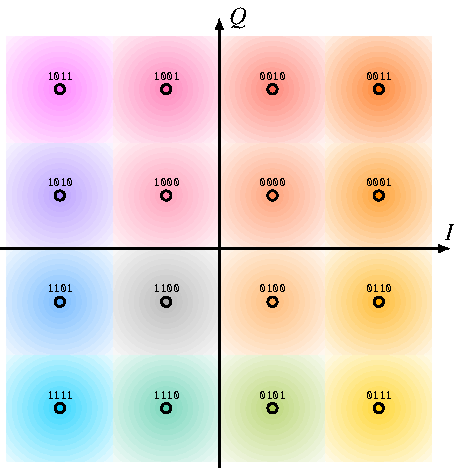
\includegraphics{applications/qam/images/konstellation.pdf}
\caption{Konstellationsdiagramm für quantisierte QAM mit 16 verschiedenen
Symbolen.
Mit jedem Symbol werden vier Bit codiert.
Zu jedem Symbol gehört ein quadratisches Gebiet gleicher Farbe.
Fällt der empfangene Vektor in eines dieser Gebiete, wird er als
das zugehörige Symbol decodiert.
\label{figure:qam:konstellation}}
\end{figure}

Im Beispiel der Abbildung~\ref{figure:qam:konstellation} können 16 
verschiedene Vektoren unterschieden werden, die man mit vierstelligen
Binärzahlen identifizieren kann.
Mit jedem Symbol werden also vier Bit übertragen.
Dieses Verfahren heisst auch 16-QAM und wird bei DVB-T verwendet.

Die Punkte-Menge $\vec{v}_k$ heisst auch die {\em Konstellation}
des Verfahrens.
Durch feinere Aufteilung können mehr Bits pro Symbol übertragen werden,
wie in Tabelle~\ref{table:qam:xqam} zusammengstellt.
Abbildung~\ref{figure:qam:analyzer} zeigt, wie sich die Messung eines 256-QAM 
Signals auf einem Vector Signal Analyzer darstellt.

Für ungerade Potenzen von $2$ kann das Konstellationsdiagramm kein
Quadrat sein.
Für $k$ ungerade kann man aber $2^k$ Punkte erhalten, indem man
dem Quadrat der $2^{k-1}$ Punkte der Konstellation von $2^{k-1}$-QAM
vier Rechtecke mit jeweils $2^{k-1}/4=2^{k-3}$ Punkten hinzugefügt, daraus
ergibt sich eine Konstellation mit
$2^{k-1}+4\cdot 2^{k-3}=2^{k-1}+2^{k-1}=2^k$
Punkten (Abbildung~\ref{qam:figure:qam-konstellation} Mitte).
In diesem hat das Konstellationsdiagramm also die Form
eines Kreuzes mit breite $2^{(k-1)/2}$ und Armlänge
$\frac32\cdot 2^{(k-1)/2}$.
Diese Konstellation wird manchmal auch Cross-QAM genannt.

\begin{table}
\centering
\begin{tabular}{rrcrl}
\hline
Bits&Symbole&Konstellation&Name&Anwendung\\
\hline
   2&      4&$  2\times   2$      &    4-QAM&DVB-S       \\
   4&     16&$  4\times   4$      &   16-QAM&V.29, DVB-T \\
   6&     64&$  8\times   8$      &   64-QAM&DVB-C, DVB-T\\
   8&    256&$ 16\times  16$      &  256-QAM&DVB-C       \\
  10&   1024&$ 32\times  32$      & 1024-QAM&            \\
  12&   4096&$ 64\times  64$      & 4096-QAM&DVB-C2, G.hn\\
  15&  32768&$128\times 256$ Kreuz&32767-QAM&ADSL        \\
\hline
\end{tabular}
\caption{Verschiedene Konstellationen für quantisierte QAM mit Anwendungen.
\label{table:qam:xqam}}
\end{table}

\begin{figure}
\centering
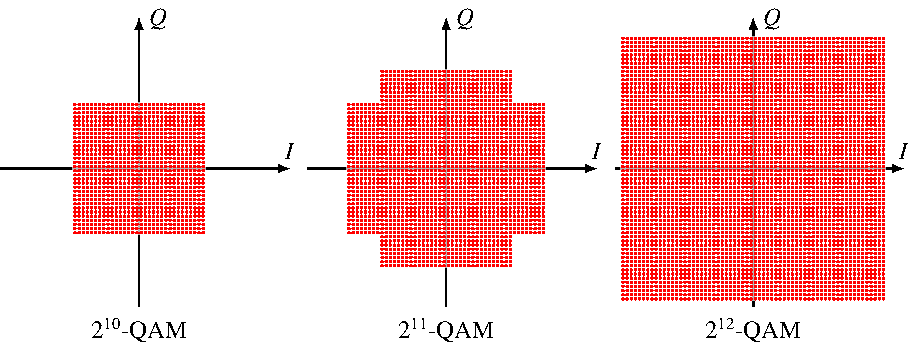
\includegraphics{applications/qam/images/qam.pdf}
\caption{Konstellationsdiagramme für $2^k$-QAM für verschiedene Werte von $k$.
\label{qam:figure:qam-konstellation}}
\end{figure}

\begin{figure}
\centering
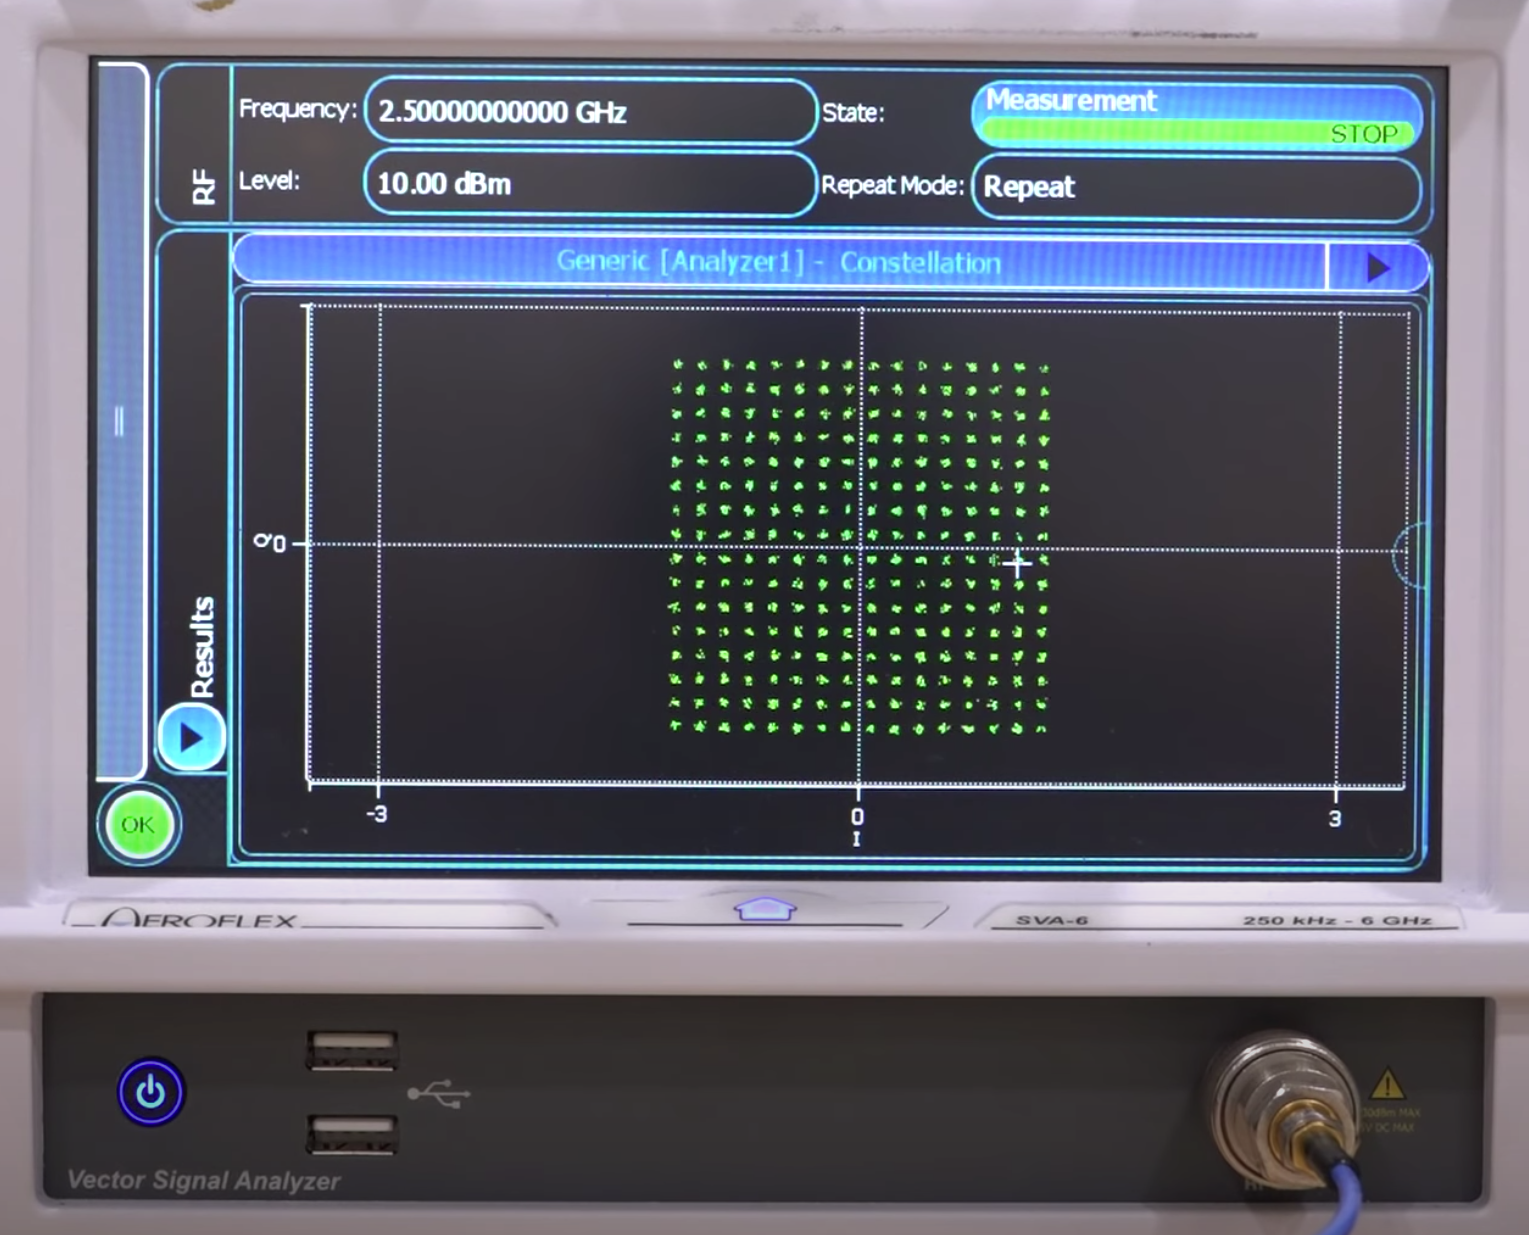
\includegraphics[width=1.0\hsize]{applications/qam/images/analyzer.png}
\caption{Messung des Konstellationsdiagramms eines 256-QAM Signals
mit einem Vector Signal Analyzer.
Man beachte die Beschriftung der Achsen mit \texttt{I} und \texttt{Q}.
(Ausschnitt aus dem Video \url{https://www.youtube.com/watch?v=uV3O3tpjmS8}
bei 26:36).
\label{figure:qam:analyzer}}
\end{figure}

\subsubsection{$n$-PSK}
Analog zum Vorgehen bei der quantisierten QAM kann auch PSK diskretisiert
werden.
Als Konstellationsdiagramm für $n$-PSK dienen $n$ Punkte auf einem Kreis,
die durch einen Winkel $2\pi/n$ getrennt sind.
In Abbildung~\ref{figure:qam:psk} ist das Konstellationsdiagramm für
$8$-PSK dargestellt.
\begin{figure}
\centering
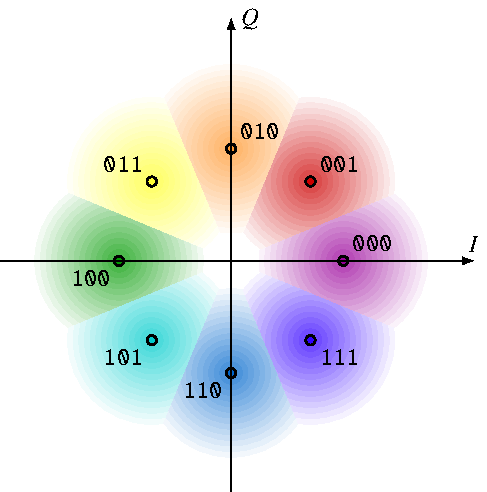
\includegraphics{applications/qam/images/psk.pdf}
\caption{Konstellationsdiagramm für 8-PSK 
\label{figure:qam:psk}}
\end{figure}

\subsubsection{Software Defined Radio}
Die vorangegangenen Beispiele haben illustriert, dass die
Quadratur-Amplituden-Modulation jedes besprochene Modulationsverfahren
realisieren kann.
Es ist nur nötig, einen Sender zu bauen, der Inputs $I(t)$ und $Q(t)$
entgegennimmt, die Modulation mit der Matrix $D_{\omega t}$ vornimmt
und das resultierende Signal $s(t)$ aussendet.
Auf der Empfängerseite braucht man eine physikalische Realisierung
der Matrix $D_{\omega_r t}$ und des Tiefpasses, der die demodulierten
Signal $\hat{I}(t)$ und $\hat{Q}(t)$ ausgibt.
Die Decodierung zum Beispiel als amplitudenmoduliertes Sprachsignal,
als frequenzmoduliertes Musiksignal oder als digitales 16-QAM-Signal
kann danach ausschliesslich in Software erfolgen.
Die Modulationsart eines solchen sogenannten {\em Software Defined Radio (SDR)}
wird also durch die Software definiert, welche die Signale $I(t)$ und $Q(t)$
erzeugt bzw.~die Signale $\hat{I}(t)$ und $\hat{Q}(t)$ analysiert.
SDR ermöglicht dem interessierten Hacker auch exotische Experimente,
wie das in Abbildung~\ref{qam:figure:digital} dargestellte fiktive
digitale Modulationsverfahren.

\begin{figure}
\centering
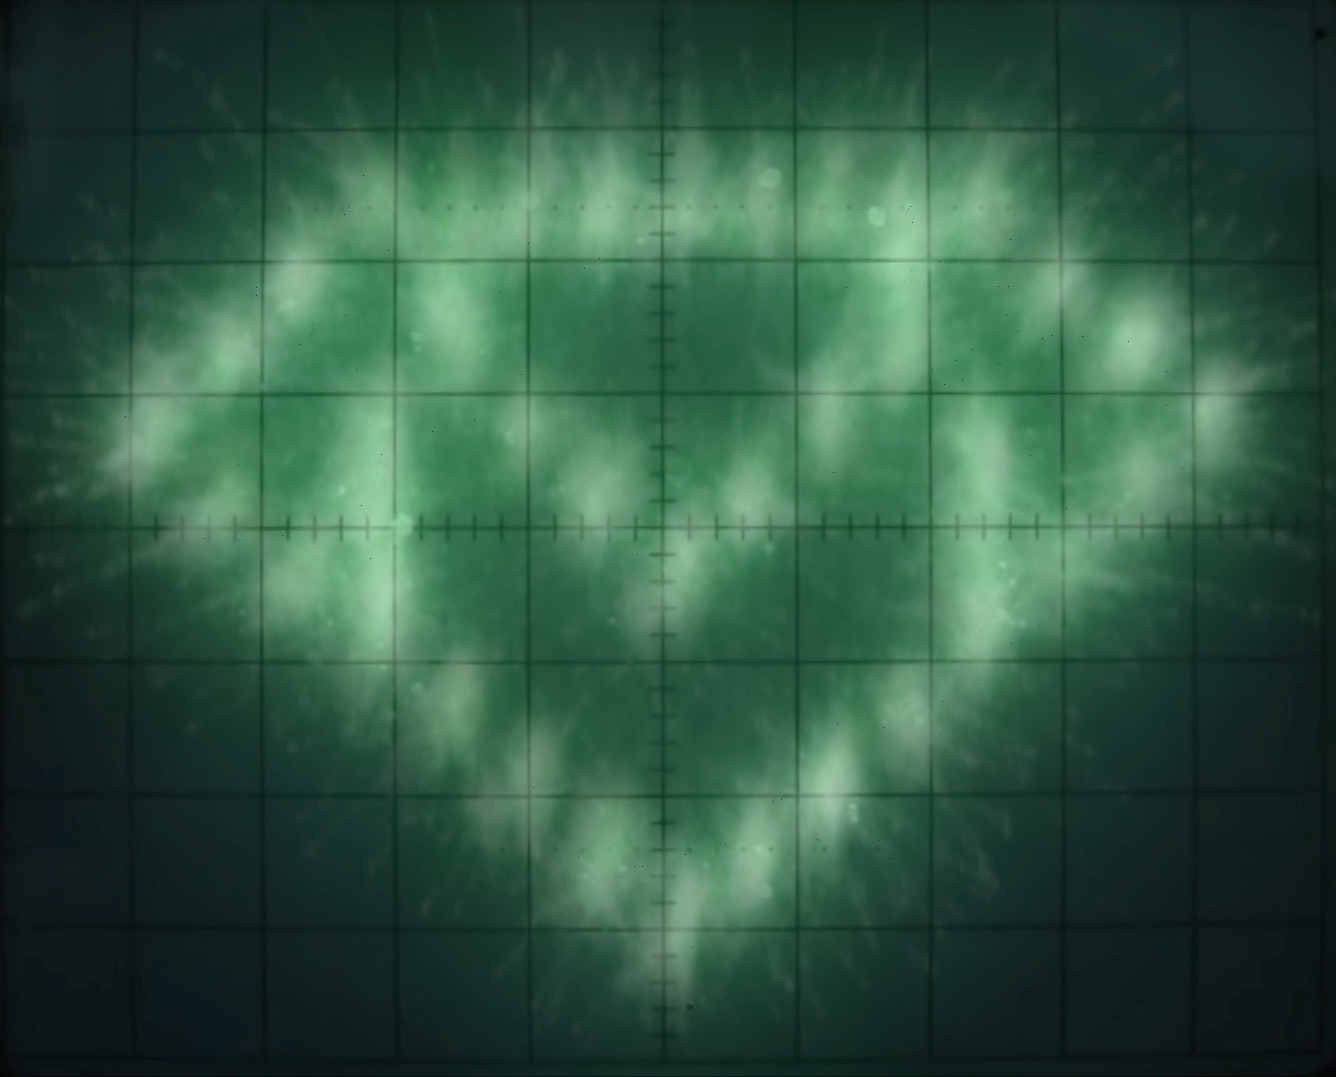
\includegraphics[width=0.7\hsize]{applications/qam/images/digital.jpg}
\caption{Konstellationsdiagramm für ein fiktives digitales
Modulationsverfahren, welches nur Punkte eines MathMan-Logos als
Symbole verwendet.
\label{qam:figure:digital}}
\end{figure}



%
% char.tex
%
% (c) 2018 Prof Dr Andreas Müller, Hochschule Rapperswil
%
\section{Charakteristische Gleichung}
\rhead{Charakteristische Gleichung}
\index{charakteristische Gleichung}
Welche Eigenwerte und Eigenvektoren hat eine Matrix? Ein Eigenvektor 
ist ein von $0$ verschiedener Vektor $x$, der die Gleichung
$Ax=\lambda x$ erfüllt, oder wie wir früher gesehen haben,
eine nicht verschwindende Lösung des homogenen Gleichungssystems
$(A-\lambda E)x=0$.
Im Kapitel \ref{chapter-determinanten} wurde gezeigt, dass ein eine solche
Lösung nur dann existieren kann, wenn die Determinante des Gleichungssystems
verschwindet, also
\[
\det(A-\lambda E)=
\left|
\begin{matrix}
a_{11}-\lambda&a_{12}&\dots&a_{1n}\\
a_{21}&a_{22}-\lambda&\dots&a_{2n}\\
\vdots&\vdots&\ddots&\vdots\\
a_{n1}&a_{n2}&\dots&a_{nn}-\lambda
\end{matrix}
\right|
\]
Die Determinante ist ein Polynom $n$-ten Grades in $\lambda$, das Finden der
Eigenwerte läuft also darauf hinaus, Nullstellen eines Polynoms zu finden.
\begin{satz}
Die Eigenwerte einer $n\times n$ Matrix $A$ sind Nullstellen des
Polynoms
\[
\chi_A(\lambda)=\det(A-\lambda E)
\]
vom Grad $n$.
\end{satz}
\begin{definition}
\index{charakteristisches Polynom}
Das Polynom $\chi_A(\lambda)=\det(A-\lambda E)$ heisst
charakteristisches Polynom,
die Gleichung $\chi_A(\lambda)=0$ heisst 
charakteristische Gleichung.
\end{definition}

\begin{beispiel}
Die Matrix $A=\begin{pmatrix}0&1\\1&0\end{pmatrix}$ hat das 
charakteristische Polynom
\begin{align*}
\det(A-\lambda I)&=\left|\begin{matrix}-\lambda&1\\1&-\lambda\end{matrix}\right|\\
&=\lambda^2-1=(\lambda+1)(\lambda-1)
\end{align*}
mit den Lösungen $\lambda_\pm=\pm1$.
Um die Eigenvektoren zu finden, muss
man jetzt das Gleichungssystem $(A-\lambda E)x=0$ bestimmen.
Für die Eigenwerte $\pm1$ hat das Gleichungssystem die Matrizen
\[
\begin{pmatrix}
-1&1\\1&-1
\end{pmatrix}\quad \text{für $\lambda=1$},\qquad
\begin{pmatrix}
1&1\\1&1
\end{pmatrix}\quad\text{für $\lambda=-1$}
\]
mit den Lösungsvektoren 
\[
\vec v_+=\begin{pmatrix}1\\1\end{pmatrix},
\qquad
\vec v_-=\begin{pmatrix}1\\-1\end{pmatrix}.
\]
\end{beispiel}


%
% diagonal.tex
%
% (c) 2018 Prof Dr Andreas Müller, Hochschule Rapperswil
%
\section{Diagonalisierung symmetrischer Matrizen\label{section-diag-sym}}
\index{Matrix!symmetrische}
Falls eine Basis aus Eigenvektoren existiert, lässt sich eine Matrix
besonders einfach als Diagonalmatrix darstellen.
Leider ist die Existenz
einer Basis aus Eigenvektoren im Allgemeinen nicht garantiert, und noch
viel weniger darf man annehmen, dass eine orthonormierte Basis
von Eigenvektoren existiert.
Im Spezialfall einer symmetrischen Matrix
ist dies jedoch immer möglich, wie in diesem Abschnitt gezeigt werden
soll.

In diesem Abschnitt sei $A$ eine symmetrische $n\times n$-Matrix,
also  $A^t=A$.

\begin{hilfssatz}
Sind $v_1$ und $v_2$ Eigenvektoren von $A$ zu den Eigenwerten 
$\lambda_1$ und $\lambda_2$ mit $\lambda_1\ne \lambda_2$, dann
ist $v_1\cdot v_2=0$.
\end{hilfssatz}

\begin{proof}[Beweis]
Wir berechnen das Skalarprodukt $v_1\cdot Av_2$ auf zwei verschiedene
Arten, wobei wir in der zweiten Variante ausnützen, dass $A=A^t$:
\begin{align*}
v_1^tAv_2&=\lambda_2v_1^tv_2
\\
v_1^tAv_2&=v_1^tA^tv_2=(Av_1)^tv_2=\lambda_1v_1^tv_2
\\
\Rightarrow
\qquad
0&=(\lambda_2-\lambda_1)v_1^tv_2
\end{align*}
Da $\lambda_2\ne\lambda_1$ ist $\lambda_2-\lambda_1\ne 0$, man kann
also durch den Klammerausdruck teilen und findet
\[
v_1^tv_2=v_1\cdot v_2=0,
\]
die beiden Eigenvektoren stehen also senkrecht aufeinander.
\end{proof}

\begin{hilfssatz}
\label{ev-ortho}
Ist $v$ ein Eigenvektor zum Eigenwert $\lambda$, und $w\perp v$ ein weiterer
Vektor, dann ist auch $Aw\perp v$.
\end{hilfssatz}

\begin{proof}[Beweis]
Wir berechnen das Skalarprodukt
\[
(Aw)\cdot v=(Aw)^t v=w^tA^tv=w^tAv=w^t\lambda v=\lambda w\cdot v=0,
\]
also $Aw\perp v$.
\end{proof}

\begin{hilfssatz}
\label{ev-existenz}
Sei $v$ ein Einheitsvektor für den $v^tAv$ den minimalen Wert $\lambda$ annimmt.
Dann ist $v$ ein Eigenvektor zum Eigenwert $\lambda$.
\end{hilfssatz}

\begin{proof}[Beweis]
Wir müssen zeigen, dass $Av=\lambda v$.
Da $v$ so gewählt war, dass $v^tAv$ minimal wird, berechnen wir 
\begin{align*}
f(t)&=\frac{(v+ty)^tA(v+ty)}{(v+ty)^t(v+ty)}
\\
&=
\frac{v^tAv+t(y^tAv+v^tAy)+t^2y^tAy}{v^tv+t(y^tv+v^ty)+t^2v^tv}
\\
f'(0)
&=
\frac{ (y^tAv+v^tAy)v^tv + v^tAv(y^tv+v^ty) }{ (v^tv)^2 }
\\
&=
\frac{ (y^tAv+v^tAy) - \lambda (y^tv+v^ty) }{ v^tv }
\\
&=
2\frac{ v^tAy - \lambda v^ty }{ v^tv }
\\
&=
2\frac{ (Av - \lambda v)^ty }{ v^tv }=0
\end{align*}
Da dies für jeden Vektor $y$ gilt, folgt $Av-\lambda v=0$, also
$Av=\lambda v$, $v$ ist also ein Eigenvektor.
\end{proof}

\begin{satz}
\label{satz:symmetrischdiagonalisierbar}
Sei $A$ eine symmetrische Matrix, dann gibt es eine orthonormierte Basis
von Eigenvektoren von $A$.
\end{satz}

\begin{proof}[Beweis]
Wir beweisen diesen Satz mit Induktion nach der Dimension des Vektorraumes.

Ein $1$-dimensionaler Raum enthält ausschliesslich Eigenvektoren.

Sei jetzt also ein Vektorraum der Dimension $n$.
Nach Hilfssatz \ref{ev-existenz} gibt es mindestens einen Eigenvektor $v_1$
zum Eigenwert $\lambda$.
Die Menge der Vektoren, die auf $v_1$ senkrecht
stehen, bilden einen Vektorraum $V_1$.
Die durch $A$ definierte Abbildung
bildet Vektoren aus $V_1$ nach Hilfssatz \ref{ev-ortho} wieder nach
$V_1$ ab.
Die Dimension von $V_1$ ist um $1$ kleiner, nach der
Induktionsannahme gibt es also ein Basis von Einheitsvektoren in $V_1$.
Damit ist auch in $V$ eine Basis aus Eigenvektoren konstruiert.
\end{proof}

\begin{beispiel} Eine symmetrische $2\times 2$-Matrix 
\[
A=\begin{pmatrix}a&b\\b&c\end{pmatrix}
\]
ist nach Satz \ref{satz:symmetrischdiagonalisierbar} diagonalisierbar.
Unter welchen Bedingungen haben die beiden Eigenwerte das gleiche
oder verschiedenes Vorzeichen?

\smallskip
{\parindent 0pt Die Eigenwerte können mit dem charakteristischen
Polynom berechnet werden:}
\[
\left|\;
\begin{matrix}a-\lambda & b\\ b&c-\lambda\end{matrix}
\;\right|=(a-\lambda)(c-\lambda)-b^2
=
\lambda^2-(a+c)\lambda+ ac-b^2=0
\]
Die zwei Eigenwerte $\lambda_1$ und $\lambda_2$ sind Nullstellen
dieses Polynoms, also gilt
\begin{align*}
(\lambda-\lambda_1)(\lambda-\lambda_2)&=\lambda^2-(\lambda_1+\lambda_2)\lambda
+\lambda_1\lambda_2=
\lambda^2-(a+c)\lambda+ ac-b^2=0\\
\Rightarrow\qquad
\lambda_1+\lambda_2&=a+c\\
\lambda_1\lambda_2&=ac-b^2
\end{align*}
Wir wählen die Bezeichnungen so, dass $\lambda_1$ der grössere Eigenwert ist.
Haben beide Eigenwerte das gleiche Vorzeichen, ist $ac-b^2>0$.
In diesem
Fall kann man das gemeinsame Vorzeichen der Eigenwerte an der Summe
$\lambda_1+\lambda_2=a+c$ ablesen.
Die Resultate sind in Tabelle
\ref{vorzeichen-eigenwerte} zusammengestellt.
\begin{table}
\begin{center}
\begin{tabular}{|>{$}c<{$}|>{$}c<{$}|>{$}c<{$}|>{$}c<{$}|}
\hline
	&a+c\ge0
		&a+c\le0
\\
\hline
ac-b^2>0
	&\lambda_1\ge\lambda_2>0
		&\lambda_2\le\lambda_1<0
\\
\hline
ac-b^2=0
	&\lambda_1\ge 0
		&\lambda_1=0
\\
	&\lambda_2=0
		&\lambda_2 \le 0
\\
\hline
ac-b^2<0
	&\lambda_1>0
		&\lambda_1>0
\\
	&\lambda_2<0
		&\lambda_2<0
\\
	&\lambda_1\ge|\lambda_2|
		&\lambda_1\le|\lambda_2|
\\
\hline
\end{tabular}
\end{center}
\caption{Vorzeichen und relative Grösse der Eigenwerte einer
symmetrischen $2\times 2$-Matrix
\label{vorzeichen-eigenwerte}}
\end{table}
\end{beispiel}

\begin{beispiel}[Zahlenbeispiel]
Welche Vorzeichen haben die Eigenwerte der symmetrische Matrix
\[
A=\begin{pmatrix}
3&4\\
4&5
\end{pmatrix}?
\]

\smallskip
{\parindent 0pt $\det(A)=-1$ und $3+5=8>0$, also kann man aus der
Tabelle \ref{vorzeichen-eigenwerte}
ablesen, dass die beiden Eigenwerte entgegengesetztes
Vorzeichen haben, und dass der negative Eigenwert betragsmässig
kleiner ist.}

Man kann die Eigenwerte natürlich auch ausrechnen.
Die charakteristische Gleichung ist 
\[
\lambda^2-8\lambda-1=0
\]
und hat die Lösungen
\[
\lambda_{1,2}=4\pm\sqrt{16+1}=\begin{cases}
4+\sqrt{17}&=\phantom{-}8.12311\\
4-\sqrt{17}&=-0.12311
\end{cases}
\]
Dies bestätigt die aus der Tabelle abgeleiteten Schlüsse.
\end{beispiel}


%
% numerisch.tex
%
% (c) 2018 Prof Dr Andreas Müller, Hochschule Rapperswil
%
\section{Numerische Lösung des Eigenwertproblems}
In der Praxis müssen meist grosse Eigenwertprobleme gelöst werden.
Das Vorgehen über das charakteristische Polynom ist dabei nicht zweckmässig,
einerseits ist es sehr aufwendig zu berechnen, andererseits ist die
Berechnung der Nullstellen eines Polynoms hohen Grades mit dem Computer
keineswegs einfach.

Ein für praktische Anwendungen besonders wichtiger Fall ist
das Eigenwertproblem für symmetrische Matrizen.
Aus Abschnitt \ref{section-diag-sym} wissen wir, dass sich symmetrische
Matrizen sogar mit einer orthonormierten Basis diagonalisieren lassen.
Es muss also eine orthogonale Matrix $T$ geben, welche $A$ auf
Diagonalform transformiert, oder $T^tAT$ muss diagonal sein.
Oder $A=TDT^t$, mit einer Diagonalmatrix $D$.
Die in Abschnitt \ref{section-svd} beschriebene Singulärwertzerlegung
liefert genau so eine Zerlegung der Matrix, die Matrix $S$ von 
Satz \ref{satz-svd} ist also die gesuchte Diagonalmatrix, die
Singulärwerte sind die Eigenwerte, und die Transformationsmatrix
entspricht den Matrizen $U$ und $V$, die in diesem Falle gleich sind:
$T=U=V$.

Die Singulärwertzerlegung ist tatsächlich die Basis vieler Implementation
von Algorithmen zur Bestimmung der Eigenwerte und Eigenvektoren.
Octave/Matlab hat aber auch eine eigene Funktion zur Berechnung der
Eigenwerte und Eigenvektoren.
\begin{beispiel}
Es sollen die Eigenwerte und Eigenvektoren der Matrix
\[
A=\begin{pmatrix}0&1\\1&0\end{pmatrix}
\]
bestimmt werden.

Die Eigenwerte sind der Rückgabewert der Funktion {\tt eig}:
\begin{verbatim}
6> eig([0,1;1,0])
ans =

  -1
   1
\end{verbatim}
Wenn man aber auch die Eigenvektoren braucht, muss man als Rückgabewert
einen Vektor anfordern:
\begin{verbatim}
> [T, D] = eig([0,1;1,0])
T =

  -0.70711   0.70711
   0.70711   0.70711

D =

Diagonal Matrix

  -1   0
   0   1
\end{verbatim}
In den Spalten der Matrix $T$ stehen die Eigenvektoren, es ist
$D=T^{-1}AT$, wie man auch mit Octave nachrechnen kann:
\begin{verbatim}
0> T^-1 * A * T
ans =

  -1   0
   0   1
\end{verbatim}
Die Matrix $T$ enthält also als Spalten genau die Eigenvektoren,
also die Vektoren einer Basis, in der $A$ diagonal wird.
\end{beispiel}
Die nächsten Abschnitte sollen jetzt aber die Frage beantworten,
wie ein solches Verfahren funktionieren kann.

\subsection{Jacobi-Verfahren}
\index{Eigenwertberechnung!mit dem Jacobi-Algorithmus}
\index{Jacobi, Carl Gustav}
\index{Jacobi-Algorithmus}
Ein einfach zu verstehender Algorithmus zur Bestimmung der Eigenwerte
ist der Jacobi-Algorithmus.
Er bestimmt eine angenäherte Matrix $T$ iterativ.
Man erhält also nicht wie bei Gauss-Algorithmus und
den Matrixzerlegungen direkt eine exakte Lösung, sondern nur eine
mehr oder weniger gute Näherungslösung, die durch weitere Iterationen
verbessert werden kann.

Die Idee ist, die Matrix $T$ aus Drehmatrizen in einer der Koordinaten-Ebenen
zusammenzusetzen.
Die Drehung um den Winkel $\alpha$ in der Ebene
$x_i$-$x_k$-Ebene hat die Matrix
\begin{equation}
D_{\alpha,i,k}=\begin{pmatrix}
1     &      &           &      &           &      &      \\
      &\ddots&           &      &           &      &      \\
      &      & \cos\alpha&      &-\sin\alpha&      &      \\
      &      &           &\ddots&           &      &      \\
      &      & \sin\alpha&      & \cos\alpha&      &      \\
      &      &           &      &           &\ddots&      \\
      &      &           &      &           &      &1     \\
\end{pmatrix}
\label{matrixd}
\end{equation}
die natürlich orthogonal ist.
Diese Drehungen heissen Givens-Rotationen.
\index{Givens-Rotation}
Ausserdem ist
$D_{\alpha,i,k}^{-1}=D_{-\alpha,i,k}$.
Jetzt versucht man mit
einer solchen Drehmatrix aus $A$ eine Matrix zu machen, die 
eher wie eine Diagonalmatrix aussieht.
Natürlich geht das
normalerweise nicht exakt, aber man kann wenigstens fordern,
dass in $A''= D^{-1}AD=D^tAD$ die Elemente $a''_{ik}=0$ sind.

Wir führen jetzt die Berechnung des Produktes durch.
Zunächst das Produkt $A'=AD$,
\[
A'
=
\begin{pmatrix}
a_{11}&\dots &a_{1i}\cos\alpha - a_{1k}\sin\alpha
		&\dots  & a_{1i}\sin\alpha+a_{1k}\cos\alpha
				&\dots	&a_{1n}\\
\vdots&      &\vdots
		&	&\vdots
				&	&\vdots\\
a_{i1}&\dots &a_{ii}\cos\alpha - a_{ik}\sin\alpha
		&\dots  & a_{ii}\sin\alpha+a_{ik}\cos\alpha
				&\dots	&a_{in}\\
\vdots&      &\vdots
		&	&\vdots
				&	&\vdots\\
a_{k1}&\dots &a_{ki}\cos\alpha - a_{kk}\sin\alpha
		&\dots  & a_{ki}\sin\alpha+a_{kk}\cos\alpha
				&\dots	&a_{kn}\\
\vdots&      &\vdots
		&	&\vdots
				&	&\vdots\\
a_{n1}&\dots &a_{1i}\cos\alpha - a_{1k}\sin\alpha
		&\dots  & a_{1i}\sin\alpha+a_{1k}\cos\alpha
				&\dots	&a_{nn}\\
\end{pmatrix}
\]
Es werden also nur die Elemente in den Spalten $i$ und $k$
verändert, und zwar gilt
\begin{equation}
\begin{aligned}
a'_{ji}&=-a_{ji}\cos\alpha-a_{jk}\sin\alpha,\\
a'_{jk}&=-a_{ji}\sin\alpha+a_{jk}\cos\alpha.
\end{aligned}
\label{dtad1}
\end{equation}
Jetzt muss noch von links mit der Matrix $D^t$
multipliziert werden, um $A''=D^tAD=D^tA'$ zu bekommen.
Dabei werden die Zeilen $i$ und $k$ modifiziert.
Die Elemente ausserhalb der Spalten $i$ und $k$ werden 
dabei zu
\begin{equation}
\begin{aligned}
a''_{ij}&=a_{ij}\cos\alpha+a_{kj}\sin\alpha,\\
a''_{kj}&=-a_{ij}\sin\alpha+a_{kj}\cos\alpha.
\end{aligned}
\label{dtad2}
\end{equation}
Die Elemente in den Spalten und Zeilen $i$ und $k$ werden
auch bei diesem zweiten Schritt abegeändert zu
\begin{equation}
\begin{aligned}
a''_{ii}&=\cos\alpha \cdot a'_{ii}+\sin\alpha \cdot a'_{ki}\\
        &=\cos\alpha\cdot (a_{ii}\cos\alpha+a_{ik}\sin\alpha)
         +\sin\alpha\cdot (a_{ki}\cos\alpha+a_{kk}\sin\alpha)\\
        &=a_{ii}\cos^2\alpha-a_{kk}\sin^2\alpha+2a_{ki}\sin\alpha\cos\alpha
\\
a''_{ki}&=-\sin\alpha \cdot a'_{ii}+\cos\alpha \cdot a'_{ki}\\
        &=-\sin\alpha\cdot (a_{ii}\cos\alpha+a_{ik}\sin\alpha)
         +\cos\alpha\cdot (a_{ki}\cos\alpha+a_{kk}\sin\alpha)\\
        &=-\sin\alpha\cos\alpha(a_{ii}-a_{kk})
        +(-\sin^2\alpha+\cos^2\alpha)a_{ki}
\\
a''_{ik}&=\cos\alpha \cdot a'_{ik} +\sin\alpha \cdot a'_{kk}\\
        &=-\cos\alpha\cdot (a_{ii}\sin\alpha+a_{ik}\cos\alpha)
         +\sin\alpha\cdot (-a_{ki}\sin\alpha+a_{kk}\cos\alpha)\\
        &=-\sin\alpha\cos\alpha(a_{ii}-a_{kk})
        +(-\sin^2\alpha+\cos^2\alpha)a_{ik}
\\
a''_{kk}&=-\sin\alpha \cdot a'_{ik}+\cos\alpha \cdot a'_{kk}\\
        &=-\sin\alpha\cdot (-a_{ii}\sin\alpha+a_{ik}\cos\alpha)
         +\cos\alpha\cdot (-a_{ki}\sin\alpha+a_{kk}\cos\alpha)\\
        &=a_{kk}\cos^2\alpha+a_{ii}\sin^2\alpha-2a_{ik}\sin\alpha\cos\alpha
\end{aligned}
\label{dtad3}
\end{equation}
Jetzt muss $\alpha$ so gewählt werden, dass $a''_{ik}=a''_{ki}=0$
wird:
\[
-\sin\alpha\cos\alpha(a_{ii}-a_{kk}) +(-\sin^2\alpha+\cos^2\alpha)a_{ik}=0.
\]
Darin erkennen wir die Doppelwinkelformeln:
\[
-\frac{a_{kk}-a_{ii}}2 \sin2\alpha +a_{ik}\cos2\alpha=0.
\]
Folglich gilt 
\begin{equation}
\tan2\alpha=\frac{2a_{ik}}{a_{ii}-a_{kk}}.
\label{tan2alpha1}
\end{equation}
\index{Halbwinkel-Formel}
Mit der Halbwinkel-Formel für den Tangens bekommt man 
\begin{equation}
\tan\alpha=\frac{\tan2\alpha}{1+\sqrt{1+\tan^22\alpha}}
\label{tan2alpha2}
\end{equation}
und daraus
\begin{align}
\sin\alpha
&=
\frac{\tan\alpha}{\sqrt{1+\tan^2\alpha}},
\\
\cos\alpha
&=
\frac{1}{\sqrt{1+\tan^2\alpha}}.
\label{tan2alpha3}
\end{align}
Insbesondere kann man die Matrix $D$ berechnen, ohne trigonometrische
Funktionen invertieren zu müssen, 

Der Algorithmus zur Diagonalisierung von $A$ läuft jetzt also
wie folgt ab:
\begin{enumerate}
\item Initialisiere $T=E$
\item Wähle ein Element $a_{ik}\ne 0$, mit $i\ne k$, welches als
nächstes zu $0$ gemacht werden soll.
\item Bestimme $\tan2\alpha$, $\tan\alpha$, $\sin\alpha$ und $\cos\alpha$
mit den Formeln (\ref{tan2alpha1}) bis (\ref{tan2alpha3}).
\item Bestimme die Matrix $D$ mit Formel (\ref{matrixd}).
\item Bestimme die Matrix $A''$ mit den Formeln (\ref{dtad1}) bis
(\ref{dtad3}).
\item Ersetze $T$ durch $TD$, $A$ durch $A''$.
\item Falls ein Ausserdiagonalelement betragsmässig $>\varepsilon$,
verwende dessen Zeile $i$ und $k$ und fahre weiter bei Schritt 3.
\end{enumerate}
Dieser Algorithmus terminiert, wenn alle Ausserdiagonalelemente 
betragsmässig $<\varepsilon$ sind.
Übrig bleibt in der Matrix
die Diagonalmatrix, mit den Eigenwerten auf der Diagonalen, 
und die Matrix $T$, welche die Eigenschaft hat, dass $T^tAT$
eine Diagonalmatrix ist.
Die Eigenvektoren stehen in den Spalten der Matrix $T$.

\subsection{Potenzmethode\label{section:potenzmethode}}
\index{Potenz-Methode}
Für den Spezialfall, dass alle Eigenwerte einer Matrix verschieden
sind, kann man ein relativ simples Lösungsverfahren angeben.
In diesem
Abschnitt sei also $A$ eine symmetrische $n\times n$-Matrix mit
verschiedenen Eigenwerten.
\subsubsection{Eigenvektoren zum dominanten Eigenwert\label{section:dominant}}
\index{Eigenwert!dominant}
Nehmen wir an, die Eigenwerte von $A$
seien der Grösse nach geordnet:
\[
|\lambda_1| > |\lambda_2| > \dots > |\lambda_n|.
\]
Seien $v_1,\dots,v_n$ die zugehörigen Eigenvektoren.
Jetzt nehmen wir einen beliebigen Vektor $u$.
Da die Eigenvektoren eine Basis bilden,
kann man $u$ in dieser Basis schreiben:
\[
u=u_1v_1+u_2v_2+\dots+u_nv_n.
\]
Wenden wir auf diesen Vektor die Matrix $A$ mehrmals an, entstehen
nacheinander
\begin{align}
Au&=
u_1\lambda_1v_1+u_2\lambda_2v_2+\dots+u_n\lambda_nv_n
\notag
\\
A^2u&=
u_1\lambda_1^2v_1+u_2\lambda_2^2v_2+\dots+u_n\lambda_n^2v_n
\notag
\\
&\vdots
\\
A^ku&=
u_1\lambda_1^kv_1+u_2\lambda_2^kv_2+\dots+u_n\lambda_n^kv_n
\label{power-method-vectors}
\end{align}
Je nach der Grösse von $\lambda_i$ wachsen dabei die einzelnen
Terme $u_i\lambda_i^kv_i$ über alle Grenzen (wenn $|\lambda_i|>1$)
oder konvergieren gegen $0$ (wenn $|\lambda_i|<1$).
Auf jeden Fall
aber wird der erste Term entweder am schnellsten wachsen (wenn $|\lambda_i|>1$)
oder am langsamsten gegen $0$ gehen (wenn $|\lambda_i|<1$).
Wenn wir also den Vektor $A^ku$ immer wieder auf Länge $1$ normieren, 
werden im Vergleich zum ersten Term alle anderen Terme gegen $0$ gehen.

\begin{beispiel}
Wir betrachten die Matrix 
\[
A=\begin{pmatrix}
1&2&3\\
2&4&5\\
3&5&6
\end{pmatrix}
\]
Die Eigenwerte sind tatsächlich sehr verschieden, Octave findet
die folgenden Werte:
\begin{verbatim}
> eig(A)
ans =

   -0.51573
    0.17092
   11.34481
\end{verbatim}
Jetzt wählen wir einen zufälligen Vektor
\begin{verbatim}
5> v = rand(3,1)
v =

   0.12634
   0.68662
   0.56531
\end{verbatim}
und wenden die Matrix $A$ wiederholt darauf an, und normieren nach
jedem Schritt sofort wieder:
\[
v_0 = v,\qquad v_{k+1}=\frac{Av_k}{|Av_k|},\; k\ge 0,
\]
in Octave kann man das durch die Befehle
\begin{verbatim}
> v3 = A * v2; v3 = v3 / norm(v3);
\end{verbatim}
erreichen.
Numerisch erhalten wir Resultate:
\[
v_1=\begin{pmatrix}
   0.32606\\
   0.59444\\
   0.73507
\end{pmatrix}
,\quad
v_2=\begin{pmatrix}
   0.32792\\
   0.59104\\
   0.73698
\end{pmatrix}
,\quad
v_3=\begin{pmatrix}
   0.32799\\
   0.59101\\
   0.73697
\end{pmatrix}
,\quad
v_4=\begin{pmatrix}
   0.32799\\
   0.59101\\
   0.73698
\end{pmatrix}
%,\quad
%v_5=\begin{pmatrix}
%   0.32799\\
%   0.59101\\
%   0.73698
%\end{pmatrix}
\]
Bei $v_5$ ist bereits keine Änderung mehr feststellbar.
Damit ist der Eigenvektor zum grössten Eigenwert gefunden, 
\end{beispiel}

\subsubsection{Weitere Eigenvektoren}
Hat man einen ersten Eigenvektor $v_1$ gefunden,
kann man das Problem verkleinern.
Die weiteren Eigenvektoren von $A$ stehen ja alle auf  $v_1$
senkrecht.
Man kann also eine Basistransformation
durchführen, so dass $e_1$ der erste Eigenvektor der transformierten
Matrix $A'$ ist, $A'$ hat die Form
\[
A'=\begin{pmatrix}
\lambda_1&0&\dots&0\\
0&*&\dots&*\\
\vdots&\vdots&\ddots&\vdots\\
0&*&\dots&*
\end{pmatrix}
=
\left(
\begin{tabular}{>{$}c<{$}|>{$}c<{$}>{$}c<{$}>{$}c<{$}}
\lambda_1&0&\dots&0\\
\hline
0&&&\\
\vdots&&A_2&\\
0&&&
\end{tabular}
\right)
\]
Um die weiteren Eigenvektoren zu finden, müssen wir das Verfahren jetzt
also nur auf den Teil $A_2$ anwenden.

Mit $A'=T^{-1}AT$ muss in der ersten Spalte von $T$
also der Vektor $v_1$ stehen.
Da die übrigen Vektoren senkrecht stehen,
können wir für $T$ eine orthogonale Matrix verwenden.
Eine solche
können wir dadurch finden, dass wir zu $v_1$ noch ein paar linear
unabhängige Vektoren hinzunehmen und darauf das Orthogonalisierungsverfahren
anwenden.

\begin{beispiel}
Wir arbeiten wieder mit der Matrix $A$ mit dem bereits berechneten
Eigenvektor v:
\[
A=\begin{pmatrix}
1&2&3\\
2&4&5\\
3&5&6
\end{pmatrix}
,\qquad
v=\begin{pmatrix}
   0.32799\\
   0.59101\\
   0.73698
\end{pmatrix}.
\]
Wir suchen jetzt eine orthogonale Transformationsmatrix $T$, die $v$
als erste Spalte hat.
Dazu füllen wir $V$ einfach mit Basisvektoren
zu einer Matrix $T_0$ auf (diese ist natürlich nicht orthogonal),
und verwenden die Orthogonalisierung, um $T$ zu erhalten.
\[
T_0=\begin{pmatrix}
   0.32799&0&0\\
   0.59101&1&0\\
   0.73698&0&1
\end{pmatrix}
\qquad\rightarrow\qquad
T=
\begin{pmatrix}
   0.32799 &-0.24030& -0.91361\\
   0.59101 &\phantom{-} 0.80666&  \phantom{-}0.00000\\
   0.73698 &-0.53995&  \phantom{-}0.40659
\end{pmatrix}
\]
Damit ist die transformierte Matrix 
\begin{align*}
A'&=T^tAT=\begin{pmatrix}
   11.345              &0.00000 & \phantom{-}0.00000\\
   \phantom{0}0.00000  &0.05740 & \phantom{-}0.25507\\
   \phantom{0}0.00000  &0.25507 &-0.40221
\end{pmatrix}
\\
\Rightarrow\qquad
A_2&=
\begin{pmatrix}
   0.05740 & \phantom{-}0.25507\\
   0.25507 &-0.40221
\end{pmatrix}
\end{align*}
Für $A_2$ kann man den nächsten Eigenvektor wieder mit der
gleichen Methode bestimmen, oder mit dem Jacobi-Verfahren.
Man findet wieder eine Matrix $T_2$, welche $A_2$ auf Diagonalform
transformiert, in diesem Fall
\[
T_2=\begin{pmatrix}
   0.91361&          -0.40659\\
   0.40659&\phantom{-}0.91361
\end{pmatrix},\qquad
T_2A_2T_2^t=
\begin{pmatrix}
   0.17092&        0\\
         0& -0.51573
\end{pmatrix}
\]
Die Eigenwerte sind damit auch bereits bekannt.
In der Matrix $T_2$ stehen in den Spalten die Eigenvektoren
von $A_2$.
Die Eigenvektoren von $A$ kann man daraus jetzt zusammensetzen:
\[
V=
T\left(
\begin{tabular}{>{$}c<{$}|>{$}c<{$}>{$}c<{$}}
1&0&0\\
\hline
0&\multicolumn{2}{c}{\raisebox{-1.5ex}[0cm][0cm]{$T_2$}}\\
0
\end{tabular}
\right)
=\begin{pmatrix}
   0.32799&            -0.59101&           -0.73698\\
   0.59101& \phantom{-} 0.73698&           -0.32799\\
   0.73698&            -0.32799& \phantom{-}0.59101
\end{pmatrix}
\]
Tatsächlich transformiert diese Matrix das ursprünglich $A$ auf
Diagonalform:
\[
V^tAV=\begin{pmatrix}
11.345&0&0\\
0&0.17092&0\\
0&0&-0.51573
\end{pmatrix}
\]
Damit haben wir alle Eigenwerte und Eigenvektoren gefunden.
\end{beispiel}

\subsection{QR-Algorithmus}
\index{Eigenwertberechnung!mit dem QR-Algorithmus}
\index{QR-Algorithmus}
Sei $A$ wieder eine symmetrische $n\times n$-Matrix.
Wir wissen aus
Abschnitt \ref{section-qr}, dass jede Matrix als Produkt $A=QR$
geschrieben werden kann, wobei $Q$ orthogonal und $R$ eine obere
Dreiecksmatrix ist.
Die erste Spalte von $Q$ ist bis auf die Länge die erste Spalte
von $A$, genauer
\[
\begin{pmatrix}a_{11}\\\vdots\\a_{n1} \end{pmatrix}
=
\begin{pmatrix}q_{11}\\\vdots\\q_{n1} \end{pmatrix}\cdot r_{11}.
\]
Die Matrix $Q$ vollzieht also eine Basistransformation
in ein Koordinatensystem, in dem der erste Basisvektor die Richtung
der ersten Spalte von $A$ hat.

Wiederholt man diese Prozedur mit
der Matrix $A_2=Q^tAQ$, findet man $A_2=Q_2R_2$, 
$Q_2$  bildet den ersten Basisvektor auf das Bild  des ersten
Basisvektors unter $A_2$ ab.
Man kann dies iterieren,
\[
A_k=Q_kR_k\quad\Rightarrow\quad
A_{k+1}=Q_k^tA_kQ_k.
\]
In jedem Schritt bildet $Q_k$ den ersten Basisvektor auf die Richtung
der ersten Spalte von $A_k$ ab.
Dieses Vorgehen unterscheidet sich
also von der Potenzmethode nur dadurch, dass man nach jeder Iteration
auch noch das Koordinatensystem wechselt.

Setzt man alle $Q_k$ zusammen, bilden
sie nacheinander den $e_1$ auf die $A^ke_1$ ab, allerdings wird
dies in jedem Schritt in einem anderen Koordinatensystem ausgedrückt.
Unter den Voraussetzungen der Potenzmethode wird die Richtung von
$A^ke_1$ gegen den dominanten Eigenvektor konvergieren.
Für $A_k$ bedeutet dies,
dass das Element in der linken oberen Ecke gegen den dominanten Eigenwert
konvergiert, und alle anderen Elemente in der gleichen Zeile und Spalte
gegen $0$.

Um das ständig wechselnde Koordinatensystem wieder zurückzurechnen,
muss das Produkt der $Q_k$ ermittelt werden,  die Matrix
\[
V=Q_1Q_2Q_3\dots
\]
enthält dann in der ersten Spalte den ersten Eigenvektor.

\begin{beispiel}
Wir gehen aus von der Matrix
\[
A=\begin{pmatrix}
6&3&5\\
3&1&2\\
5&2&4
\end{pmatrix},
\]
einer permutierten Variante der bisher betrachteten Matrix.
Die QR-Zerlegung liefert
\[
Q=\begin{pmatrix}
   0.71714&  \phantom{-}0.65809& -0.22942\\
   0.35857& -0.63067& -0.68825\\
   0.59761& -0.41131& \phantom{-}0.68825
\end{pmatrix},
\quad
R=\begin{pmatrix}
   8.36660&  3.70521&  6.69328\\
   0.00000&  0.52099&  0.38389\\
   0.00000&  0.00000&  0.22942
\end{pmatrix}
\]
Die transformierte Matrix $A_2$ ist dann
\[
A_2=Q^tAQ=\begin{pmatrix}
   11.328571&  \phantom{-}0.416226&  \phantom{-}0.137102\\
    0.416226&  -0.486466&  -0.094360\\
    0.137102&  -0.094360&  \phantom{-}0.157895
\end{pmatrix}
\]
Der dominante Eigenwert in der linken oberen Ecke der Matrix zeichnet
sich bereits ab.
Iteriert man jetzt, und rechnet auch immer gleich
das Produkt $U_k=Q_1\dots Q_{k-1}$ aus, findet man nacheinander
\begin{align*}
A_3&=\begin{pmatrix}
             11.345\phantom{00}&  \phantom{-}0.01958&   \phantom{-}0.00209\\
   \phantom{0}0.01958          &  -0.51406&  -0.03348\\
   \phantom{0}0.00209          &  -0.03348&  \phantom{-}0.16928
\end{pmatrix}&
U_3&=\begin{pmatrix}
   0.73799& -0.57307& -0.35631\\
   0.32682& \phantom{-}0.76549& -0.55427\\
   0.59039& \phantom{-}0.29259& \phantom{-}0.75222
\end{pmatrix}
\\
A_4&=\begin{pmatrix}
   11.345\phantom{00} &  \phantom{-}0.00089&  \phantom{-}0.00003\\
   \phantom{0}0.00089& -0.51555& -0.01112\\
   \phantom{0}0.00003& -0.01112&  \phantom{-}0.17074
\end{pmatrix}&
U_4&=\begin{pmatrix}
   0.73693&  \phantom{-}0.59630& -0.31837\\
   0.32804& -0.72728& -0.60287\\
   0.59103& -0.33983&  \phantom{-}0.73157
\end{pmatrix}
\\
A_5&=\begin{pmatrix}
   11.345\phantom{00}&  \phantom{-}0.00004&  \phantom{-}0.00000\\
   \phantom{0}0.00004& -0.51571& -0.00368\\
   \phantom{0}0.00000& -0.00368&  \phantom{-}0.17090
\end{pmatrix}&
U_5&=\begin{pmatrix}
   0.73698& -0.58924& -0.33115\\
   0.32798&  0.74014& -0.58704\\
   0.59101&  0.32403&  0.73873
\end{pmatrix}
\\
%A_6&=\begin{pmatrix}
%   1.1345e+01&  1.8466e-06&  7.1446e-09\\
%   1.8466e-06& -5.1573e-01& -1.2216e-03\\
%   7.1446e-09& -1.2216e-03&  1.7091e-01
%\end{pmatrix}&
%U_6&=\begin{pmatrix}
%   0.73698&  0.59159& -0.32693\\
%   0.32799& -0.73592& -0.59232\\
%   0.59101& -0.32930&  0.73639
%\end{pmatrix}
%\\
%A_7&=\begin{pmatrix}
%   1.1345e+01&  8.3945e-08&  1.0764e-10\\
%   8.3945e-08& -5.1573e-01& -4.0484e-04\\
%   1.0764e-10& -4.0484e-04&  1.7091e-01
%\end{pmatrix}&
%U_7&=\begin{pmatrix}
%   0.73698& -0.59082& -0.32833\\
%   0.32799&  0.73732& -0.59057\\
%   0.59101&  0.32755&  0.73717
%\end{pmatrix}
&\vdots
&&\vdots
\\
A_\infty&=\begin{pmatrix}
   11.345& 0&0\\
   0& -0.51573&0\\
   0& 0&  0.17092
\end{pmatrix}&
U_\infty&=\begin{pmatrix}
   0.73698& \phantom{-}0.59101& -0.32799\\
   0.32799& -0.73698& -0.59101\\
   0.59101& -0.32799& \phantom{0}0.73698
\end{pmatrix}
\end{align*}
Man beachte, dass im Laufe des Verfahrens der zweite Eigenvektor
immer wieder sein Vorzeichen wechselt.
Der Algorithmus hat also die Eigenwerte in der Reihenfolge
ihres Betrages geliefert, die zugehörigen Eigenvektoren
stehen in den Spalten von $U_\infty$.
\end{beispiel}

Die Berechnung von $Q_k^tA_kQ_k$ ist ziemlich aufwendig, weil dazu
zwei Matrizenprodukte ausgerechnet werden müssen.
Man kann die
Berechnung allerdings drastisch vereinfachen, wenn man beachtet,
dass wegen $Q_k^tQ_k=E$ gilt
\[
A_{k+1}=Q_k^tA_kQ_k=Q_k^tQ_kR_kQ_k=R_kQ_k.
\]
Die Berechnung von $A_{k+1}$ ist also mit nur einer Matrizenmultiplikation
möglich, und noch dazu ist der eine Faktor eine Dreiecksmatrix, was den
Aufwand nochmals ungefähr halbiert.

\subsection{Verbesserungen}
Der in \ref{section-qr} beschriebene Algorithmus funktioniert, ist
aber numerisch nicht sehr zuverlässig.
Das Problem ist, dass fast
linear abhängige Vektoren zu kleinen Nennern führen, so dass
Rundungsfehler aufgeblasen werden.
Mit sogenannten Householder-Transformationen kann jedoch eine 
Verbesserung erreicht werden.
\index{Householder-Transformation}

Der QR-Algorithmus zur Eigenwert-Bestimmung ist noch nicht optimal.
Zunächst funktioniert er in dieser Form nur, wenn die Eigenwerte
verschieden und reell sind.
Selbst für symmetrische Matrizen,
für die die Eigenwerte reell sind, ist nicht ausgeschlossen, dass
Eigenwerte gleich oder fast gleich sind, was zu langsamer
Konvergenz des Algorithmus führt.

\index{Francis-Algorithmus}
Der Francis-Algorithmus korrigiert diese Defekte:
\begin{enumerate}
\item
Statt die Matrix $A$ anzuwenden, wendet er $p(A)$ an, wobei
$p(x)$ ein geeignet zu wählendes Polynom ist.
Statt (\ref{power-method-vectors}) bekommt man dann
\[
u_1p(\lambda_1)^kv_1+u_2p(\lambda_2)^kv_2+\dots+u_np(\lambda_n)^kv_n
\]
Sorgt man dafür, dass die Werte von $p(\lambda_i)$ sich stark
unterscheiden, wird die Konvergenz beschleunigt.

Man kann dies zum
Beispiel dadurch erreichen, dass man für $p$ einen Faktor des
charakteristischen Polynoms von $A$ wählt.
\item 
Damit die Konvergenz des Verfahrens schnell ist, sollte das Problem
möglichst schnell in kleinere Teilaufgaben zerlegt werden können,
die effizienter lösbar sind.
Der Francis-Algorithmus erkennt 
Blöcke, in denen die Konvergenz bereits soweit fortgeschritten
ist, dass sie sich abspalten lassen.
\item
Die Eigenwerte reeller Matrizen sind reell oder konjugiert komplexe
Paare.
Der Francis-Algorithmus erkennt $2\times 2$-Blöcke, die zu
solchen Paaren gehören, und berechnet Eigenwerte und Eigenvektoren
mit Hilfe des charakteristischen Polynoms und dem Gauss-Algorithmus.
\end{enumerate}


\section{Anwendungen}
%
% Anwendung: Google-Pagerank
%
% (c) 2012 Prof Dr Andreas Mueller
% $Id$
%
\subsection{Google Pagerank}
\index{Pagerank}
\index{Google}
\index{Suchbegriff}
\index{Suchmaschine}
Es gibt viel mehr Web-Seiten als es m"ogliche Suchw"orter gibt, jede Web-Suche
liefert notwendigerweise Tausende wenn nicht Millionen von Treffern.
Welche Seiten soll man dem Benutzer der Suchmaschine auf der ersten Seite 
anzeigen?

\subsubsection{Wahrscheinlichkeitsmodell des Internets}
\index{Internet}
\index{Link}
Googles Antwort auf dieses Problem ist: man fragt das Internet!
Ob eine Web-Seite interessant ist entscheiden die Internet-User dadurch,
dass sie auf ihren eigenen Seiten Links darauf setzen. Je mehr Links auf
eine Seite zeigen, desto bedeutender ist sie.
\begin{figure}
\[\UseTips
\entrymodifiers={++[o][F]}
\xymatrix @=1.5cm {
1 \ar[r] \ar[d]
	& 3 \ar[r] \ar[dl]
		& 5 \ar[d] \ar@/^/[r] \ar[rd]
			& 7 \ar@/^/[d]  \ar@/^/[l]
                                \ar `ul^l[lll]+/u6mm/`l^dl[lll] [lll]
\\
2 \ar@/^/[r]
	& 4 \ar@/^/[l] \ar[r] \ar[ur]
		& 6 \ar@/^/[r]
			& 8 \ar@/^/[l] \ar@/^/[u]
}
\]
\caption{Beispiel-Internet\label{google-sample}}
\end{figure}%

Die bedeutendste Seite ist diejenige, die von den meisten Benutzern
besucht wird. Nummerieren wir alle Internet-Seiten von $1$ bis $n$,
k"onnen wir die Besuchs\-h"aufigkeiten $p_i$ aller Seiten in einem
Vektor
\[
p=\begin{pmatrix}p_1\\\vdots\\p_n\end{pmatrix}
\]
zusammenfassen. In regelm"assigen Zeitabst"anden verlassen Benutzer
die Seiten, die sie gerade am Lesen sind, und klicken sich weiter zu
anderen Seiten. Die Benutzer verteilen sich neu, sie besuchen jetzt mit
H"aufigkeit $p_i'$ die Seite $i$.
Dabei folgen sie nat"urlich den Links.
Gibt es auf einer Seite $k$ Links, nehmen wir an, dass die Benutzer
zu gleichen Teilen diesen Links folgen.
Im Beispiel-Internet nach Abbildung~\ref{google-sample} gibt es drei
Links, die von Seite 5 abgehen.
Die Benutzer, die die Seite 5
besuchen, klicken sich weiter zu je einem Drittel auf die
Seiten 6, 7 und 8.
Daraus kann man jetzt die H"aufigkeit ausrechnen, mit der die
einzelnen Seiten nach dem Weiterklicken besucht werden.
Die Besucher, die nach dem Klicken auf Seite $8$ landen, rekrutieren
sich von den Seiten 5, 6 und 7:
\[
p_8'=\frac13p_5+p_6+\frac13p_7.
\]
Der Vektor $p'$ kann aus dem Vektor $p$ mit einer Matrix
\[
H=\begin{pmatrix}
%     1 2       3       4       5 6       7       8
      0&0&      0&      0&      0&0&\frac13&      0\\
\frac12&0&\frac12&\frac13&      0&0&      0&      0\\
\frac12&0&      0&      0&      0&0&      0&      0\\
      0&1&      0&      0&      0&0&      0&      0\\
      0&0&\frac12&\frac13&      0&0&\frac13&      0\\
      0&0&      0&\frac13&\frac13&0&      0&\frac12\\
      0&0&      0&      0&\frac13&0&      0&\frac12\\
      0&0&      0&      0&\frac13&1&\frac13&0\\
\end{pmatrix}
\]
nach der Formel $p'=Hp$ berechnet werden. Man beachte, dass sich die
Elemente in jeder Spalte von $H$ zu $1$ summieren.

Nat"urlich "andert sich die Beliebtheit einer Webseite viel langsamer
als die Klicks Zeit brauchen, also sollten sich die H"aufigkeiten
$p_i'$ von den H"aufigkeiten $p_i$ nicht unterscheiden:
\[
p=Hp.
\]
Insbesondere ist $p$ ein Eigenvektor zum Eigenwert $1$.

Im Beispiel-Internet findet man f"ur den Eigenvektor numerisch
\[
p=
\begin{pmatrix}
   0.077670\\
   0.087379\\
   0.038835\\
   0.087379\\
   0.247573\\
   0.150485\\
   0.233010\\
   0.077670\\
\end{pmatrix}.
\]
Seite  5 ist also die beliebteste, gefolgt von Seite 7 und 6.

\subsubsection{Freier Wille}
\index{freier Wille}
Das Modell, dem die Matrix $H$ zu Grunde liegt, ber"ucksichtigt
noch nicht, dass einige Benutzer eine Seite nicht dank der Links
finden, sondern weil sie von ihrem freien Willen gebrauch machen,
im URL-Feld des Browsers einen beliebigen URL einzugeben.
Ohne weitere Informationen m"ussen wir annehmen, dass auf diesem
Wege die Benutzer jede beliebige Seite anspringen k"onnen.
W"are dies der einzige Mechanismus, mit dem man andere Seiten erreichen
kann, dann w"are
\[
p'=\frac1n\begin{pmatrix}
1\\\vdots\\1
\end{pmatrix}.
\]
Wir m"ochten dies aber wieder in der Form $p'=Mp$ schreiben.
Da die $p_i$ sich zu $1$ summieren, gilt
\[
\begin{pmatrix}
     1&     1&\dots &     1\\
     1&     1&\dots &     1\\
\vdots&\vdots&\ddots&\vdots\\
     1&     1&\dots &     1
\end{pmatrix}
p=\begin{pmatrix}1\\1\\\vdots\\1\end{pmatrix}.
\]
Wir bezeichnen die Matrix aus lauter Einsen mit $A$, dann ist
\[
p'=\frac{1}{n}Ap.
\]

Wir f"ugen jetzt die Matrix $H$ mit dem freien Wille zusammen zur 
sogenannten Google-Matrix.
\begin{definition}
Die Matrix 
\[
G=(1-\alpha)H+\frac{\alpha}nA
\]
heisst Google-Matrix.
Der Eigenvektor zum Eigenwert $1$ heisst Google Pagerank.
\end{definition}
\index{Pagerank}
\index{Google-Matrix}
Je gr"osser der Wert $\alpha$ gew"ahlt wird, desto bedeutender wird die
Komponente des freien Willens. F"ur $\alpha=0$ ist $G=H$.

F"ur das Beispiel-Internet verschiebt sich die Beliebtheit jetzt ein bisschen,
f"ur $\alpha = 0.1$ zum Beispiel bekommen wir f"ur den Pagerank-Vektor
\[
p=\begin{pmatrix}
   0.077241\\
   0.099007\\
   0.047258\\
   0.101606\\
   0.233925\\
   0.147918\\
   0.215804\\
   0.077241
\end{pmatrix}.
\]
Die Seite 5 ist zwar immer noch die beliebteste, aber sie ist etwas zur"uckgefallen,
daf"ur ist jetzt Seite 7 etwas beliebter geworden.

\subsubsection{Bestimmung des Eigenvektors}
Die Google-Matrix ist nur dann praktisch anwendbar, wenn es eine
M"oglichkeit gibt, den Pagerank-Vektor auch dann zu berechnen, wenn $n$
sehr gross ist, also von der Gr"ossenordnung $10^{10}$.

Tats"achlich ist bekannt, dass jeder andere Eigenwert deutlich kleiner als $1$
ist.
Die Potenzmethode von Abschnitt \ref{section:dominant} ist anwendbar,
da der gesuchte Eigenvektor der Eigenvektor zum dominanten Eigenwert
ist.
Man muss also nur mit einer m"oglichst guten Approximation von $p_0$ beginnen,
und dann die Matrix $G$ mehrmals wiederholt darauf anwenden, 
\[
p_1=Gp_0,\quad
p_2=Gp_1,\quad
p_3=Gp_2,\quad\dots p_k=Gp_{k-1}=G^kp.
\]
Google verf"ugt nat"urlich immer "uber eine gute erste Approximation $p_0$:
den Pagerank-Vektor aus der letzten Berechnung.
Alle paar Tage oder Wochen berechnet Google den Pagerank-Vektor neu,
wobei sich die Reihenfolge der Suchresultate nat"urlich ver"andern
kann. Webmaster nennen dieses Ph"anomen den Google-Dance. 



